Nesta seção serão relatadas as atividades desenvolvidas pelo aluno bolsista nesta segunda metade do projeto. A seção \ref{sec:extracao} descreve o processo de extração dos pontos importantes da curva discreta obtida da imagem. A seção \ref{sec:combinacao} contém o que foi desenvolvido na etapa de combinação dos algoritmos, com a respectiva fonte para os códigos desenvolvidos. Por último, a etapa \ref{sec:avaliacao} ilustra os resultados obtidos, nos diferentes tipos de imagens e malhas utilizados para os testes.

\section{Extração dos pontos importantes}\label{sec:extracao}

A extração de pontos importantes consistem em, a partir de um conjunto finito de $n$ pontos, que representa uma curva discreta, computar os índices dos pontos âncora que serão utilizados pelo algoritmo de reconstrução. A quantidade de pontos a serem escolhidos também é enviada por parâmetro.

Alguns métodos foram considerados para a seleção dos pontos importantes. Foram eles:

\begin{itemize}
    \item \textbf{Pontos linearmente espaçados:} os pontos são escolhidos de modo que os índices sejam igualmente espaçados entre si.
    \item \textbf{Escolha aleatória de pontos:} os pontos são escolhidos de modo aleatório, apenas tomando cuidado para que não sejam muito próximos um do outro.
    \item \textbf{Escolha de pontos pela curvatura:} inicialmente é calculada a curvatura discreta da curva em cada ponto, e aqueles com maior valor absoluto são escolhidos.
\end{itemize}

Destes, serão analisados resultados encontrados utilizando pontos linearmente espaçados e pela curvatura. A escolha de pontos igualmente espaçados pode ser realizada facilmente utilizando a função \texttt{linspace} em linguagens como Python e MATLAB. Já para a escolha de pontos pela curvatura é previamente necessária a análise da curva discreta. Para isso, será revisada a teoria da análise de curvatura discreta.

A curvatura de uma curva regular parametrizada por uma aplicação $t \rightarrow (x(t), y(t))$, onde $x(t)$ e $y(t)$ são funções de classe $C^2$, é dada por \cite{OliveiraMarroquim2020}:

\begin{equation}
	\kappa (t) = \frac{x'(t) y''(t) - y'(t) x''(t)}{(x'(t)^2 + y'(t)^2)^{3/2}}.
\end{equation}

No projeto, as curvas não são contínuas, mas sim representadas por um conjunto discreto de pontos $(x, y)$ - que representam a posição de cada pixel. Por isso, as derivadas mostradas na equação acima devem ser calculadas de maneira discreta. Uma das maneiras de se calcular isto é partir de métodos espectrais de Fourier \cite{brethwashington}.

Seja $u_j$ uma aproximação discreta da função $u(x)$, com $n$ pontos de amostra $x_j \in h, 2h, \dots, ih, \dots, 2\pi - h, 2\pi$, onde $h = 2\pi/n$. Para o caso discreto, pode-se aplicar a versão computacionalmente otimizada da transformada de Fourier (FFT) em $u_j$, tal que $FFT(u_j) \equiv \hat{u}_k$, em que $k \in \frac{-n}{2}+1, \dots, \frac{n}{2}$. Sabe-se que:

$$FFT \left (\frac{\partial u_j}{\partial x} \right) \equiv i k \hat{u}_k$$

Assim, para obter o valor da derivada, basta calcular a transformada rápida inversa IFFT. O código calcula a derivada de uma função discreta $y$ no domínio $x$ e emprega um filtro Gaussiano com fator de suavização $\sigma$. A aplicação de um filtro Gaussiano no cálculo da derivada tem por objetivo evitar a amplificação do efeito de serrilhamento (\textit{aliasing}), quando houver, causado pela transformada de Fourier \cite{li1987}. O filtro Gaussiano cumpre este objetivo ao eliminar altas frequências presentes no sinal com a propriedade de preservar a localização de pontos importantes da mudança da curvatura \cite{tomasi2007}.

Com a curvatura de cada ponto calculada, é necessário escolher os pontos que serão utilizados como âncoras para representar a curva. Porém, uma  escolha simples dos pontos com maior curvatura pode fazer com que algumas regiões do contorno sejam super-representadas, enquanto outras fiquem sem pontos âncora.

Por isso, a estratégia utilizada foi a seguinte: 25\% dos pontos serão escolhidos de forma linear. Os outros 75\% serão enfim escolhidos por possuírem maior valor absoluto de curvatura. Para que os pontos sejam mais bem distribuídos por todo o contorno, antes de um ponto ser adicionado é feita uma verificação se este possui algum vizinho muito próximo presente no conjunto de pontos âncora já escolhidos. Caso o ponto não tenha vizinhos já adicionados no conjunto de pontos escolhidos, este pode ser então adicionado. A quantidade de vizinhos a serem analizados é constantemtente subtraída para que não haja laços de repetição infinitos. O trecho de código fonte abaixo descreve este processo.

\begin{lstlisting}[language=Python]
# calculo da curvatura e ordenacao dos pontos por isso
kappa = calc_curvature(contour[:,0], contour[:,1], np.arange(n))
arr = sorted([(np.abs(kappa[i]), i) for i in range(n)], reverse=True)

# escolha de 25% dos pontos de forma linear
chosen = set(np.linspace(0, n - 1, qtt//4).astype(int))

# inicia com um range maior e depois diminui
delta_range = n // 20
while len(chosen) < qtt:
  for curv, idx in arr:
    can_be = len(chosen) < qtt

  # verifica se vizinhos proximos ja estao adicionados
  for delta in range(-delta_range, delta_range):
    can_be = can_be and not (idx + delta) % n in chosen

  # pode ser adicionado no conjunto
  if can_be:
    chosen.add(idx)

  # diminui o intervalo de verificacao (evitar loops infinitos)
  delta_range = max(delta_range - 5, 0)
\end{lstlisting}

\section{Combinação dos algoritmos}\label{sec:combinacao}

Nesta seção do projeto foi implementado um \textit{notebook} em Python que organiza todas as etapas de desenvolvimento do projeto. A versão final \cite{Fakhoury2021} foi disponibilizada no GitHub\footnote{Disponível em <https://github.com/andrefakhoury/image-curve-reconstruction>. Acesso em 8 out 2021.}.

Em grande parte, os procedimentos que envolvem imagens foram tratados com a biblioteca \citeonline{OpenCV}. As operações matriciais foram resolvidas utilizando NumPy e os gráficos feitos com a biblioteca MatPlotLib.

O \textit{notebook} está organizado nas seguintes seções:

\begin{itemize}[noitemsep]
\item \textbf{Pré-processamento} - incluindo a extração dos contornos;
\item \textbf{Processamento de curvas} - a partir do conjunto de coordenadas $(x, y)$ de cada ponto, pode ser calculada a curvatura discreta;
\item \textbf{Escolha dos pontos âncora} - possibilidade de escolha dos pontos como descrito na seção anterior (\ref{sec:extracao});
\item \textbf{Reconstrução} - funções de reconstrução descritas em \citeonline{Sorkine2006};
\item \textbf{Testes} - finalmente, avaliações e testes, como serão descritas na seção \ref{sec:avaliacao}.
\end{itemize}

\section{Avaliação e testes}\label{sec:avaliacao}

Na etapa final do projeto foram realizados testes com diversas imagens, curvas e malhas. Primeiramente serão descritas as análises utilizando as imagens de folhas do repositório \citeonline{imageclef2011} - inicialmente descrito no projeto como o banco de dados a ser testado - e, posteriormente, testes em curvas abertas e fechadas em $\mathbb{R}^2$ e $\mathbb{R}^3$. Também foram realizados testes em malhas poligonais, que serão descritos no último tópico desta seção.

O erro será computado como sendo a distância euclidiana entre cada ponto da curva original e da curva reconstruída: para cada índice de vértice $i$, o erro dos pontos obtidos $\mathbf{v'}$ em relação aos pontos originais $\mathbf{v}$ é:

$$E_i(\mathbf{v, v'}) = \sqrt{(\mathbf v_i^{(x)} - \mathbf v_i'^{(x)})^2 + (\mathbf v_i^{(y)} - \mathbf v_i'^{(y)})^2}$$

\noindent e o erro total da reconstrução é calculado como a soma dos erros para cada ponto:

$$E(\mathbf{v, v'}) = \sum_{i = 1}^{|V|}E_i(\mathbf{v, v'})$$

\subsection{Imagens de folhas do repositório \citeonline{imageclef2011}}

Os primeiros exemplos analisados foram imagens de folhas de árvores, retiradas do repositório do \citeonline{imageclef2011}. Este banco de imagens foi citado no projeto original, e utilizado com a justificativa de que os contornos das figuras podem ser extraídos com alta precisão, facilitando a avaliação do método.


\begin{figure}[H]
	\centering
	\begin{subfigure}[b]{\textwidth}
		\centering
		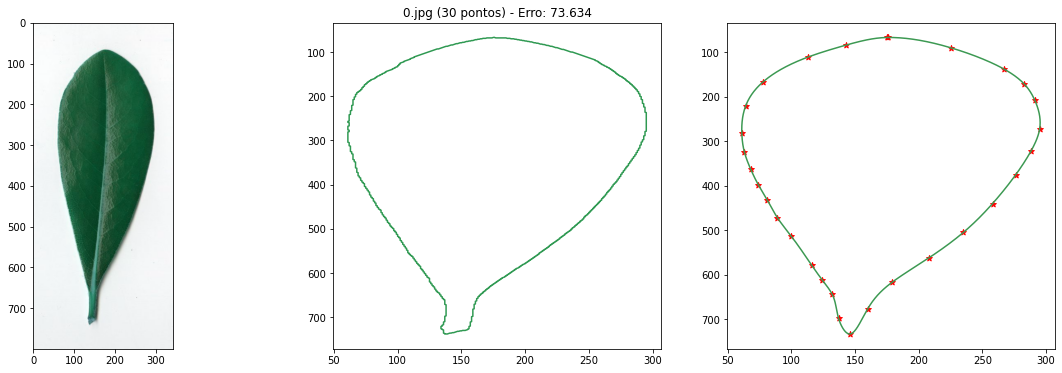
\includegraphics[width=0.9\textwidth]{img/res/0_30.png}
		\caption{Erro = 73.63.}
	\end{subfigure}
	\\
	\begin{subfigure}[b]{\textwidth}
		\centering
		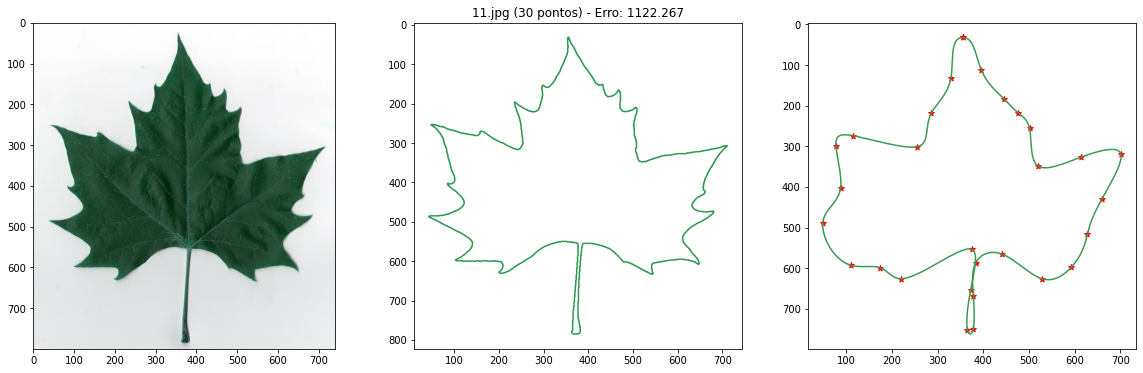
\includegraphics[width=0.9\textwidth]{img/res/1_30.png}
		\caption{Erro = 1122.27.}
	\end{subfigure}
	\\
	\begin{subfigure}[b]{\textwidth}
		\centering
		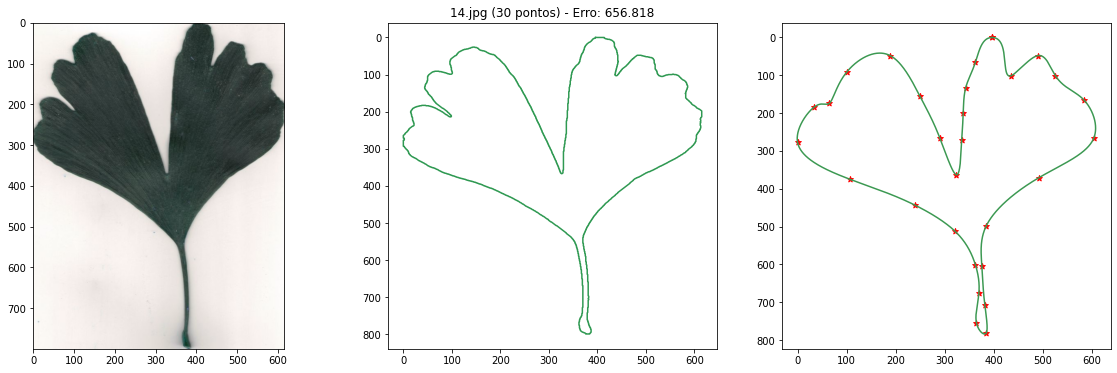
\includegraphics[width=0.9\textwidth]{img/res/2_30.png}
		\caption{Erro = 658.82.}
	\end{subfigure}
	\\
	\begin{subfigure}[b]{\textwidth}
		\centering
		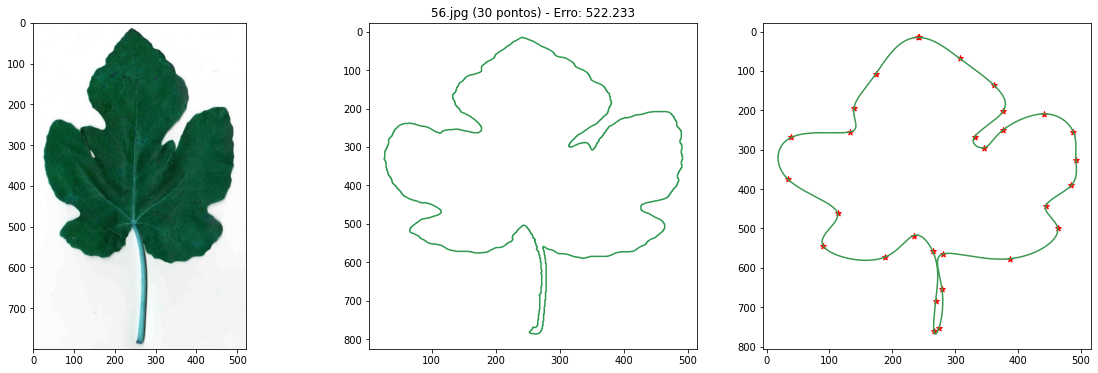
\includegraphics[width=0.9\textwidth]{img/res/3_30.png}
		\caption{Erro = 522.23.}
	\end{subfigure}
	\caption{Representação de folhas utilizando apenas 30 pontos como âncora.}
	\label{fig:folha1rep}
\end{figure}


\begin{figure}[H]
	\centering
	\begin{subfigure}[b]{\textwidth}
		\centering
		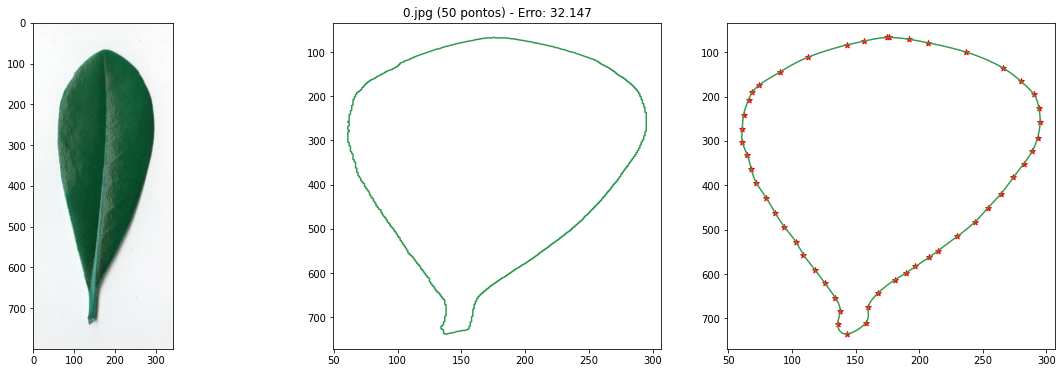
\includegraphics[width=0.9\textwidth]{img/res/0_50.png}
		\caption{Erro = 32.15.}
	\end{subfigure}
	\\
	\begin{subfigure}[b]{\textwidth}
		\centering
		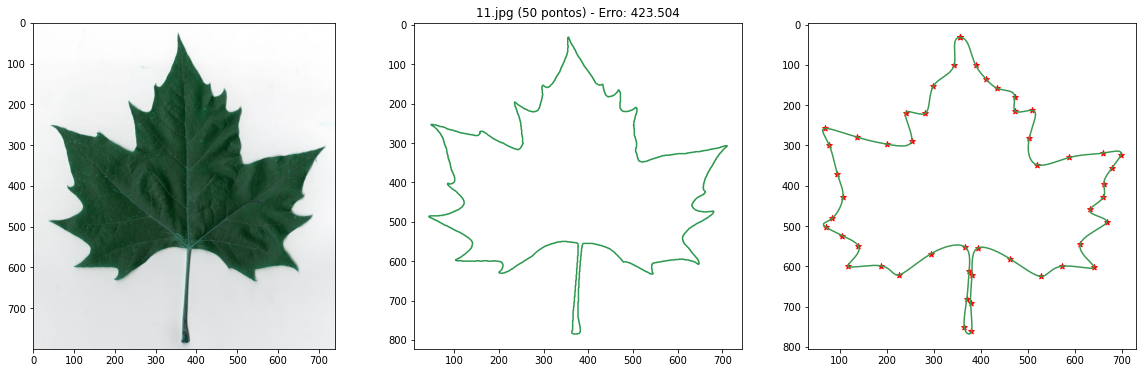
\includegraphics[width=0.9\textwidth]{img/res/1_50.png}
		\caption{Erro = 423.50.}
	\end{subfigure}
	\\
	\begin{subfigure}[b]{\textwidth}
		\centering
		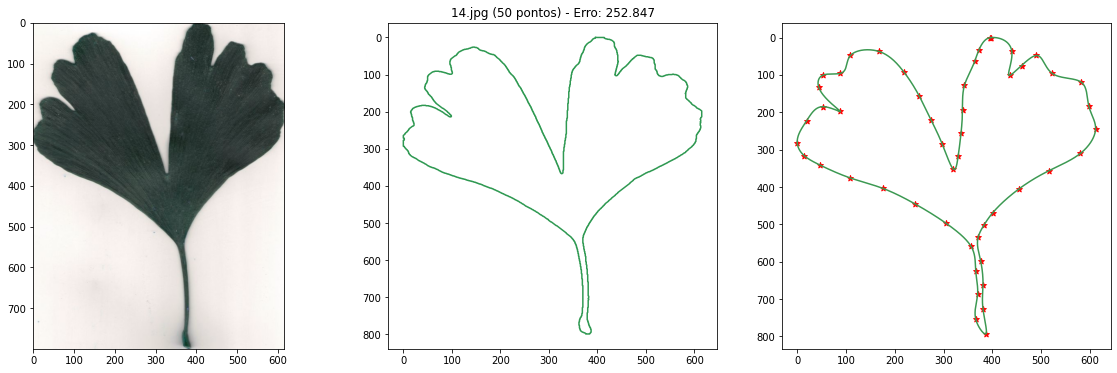
\includegraphics[width=0.9\textwidth]{img/res/2_50.png}
		\caption{Erro = 252.85.}
	\end{subfigure}
	\\
	\begin{subfigure}[b]{\textwidth}
		\centering
		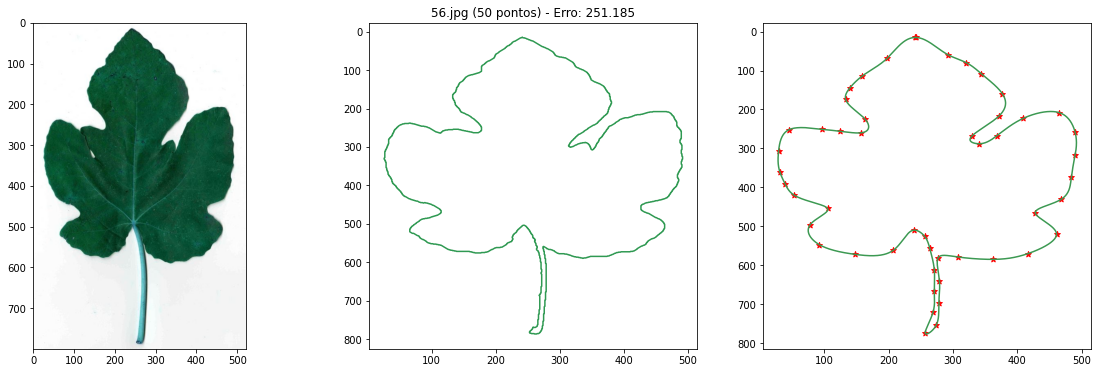
\includegraphics[width=0.9\textwidth]{img/res/3_50.png}
		\caption{Erro = 251.18.}
	\end{subfigure}
	\caption{Representação de folhas utilizando apenas 50 pontos como âncora.}
	\label{fig:folha2rep}
\end{figure}


\begin{figure}[H]
	\centering
	\begin{subfigure}[b]{\textwidth}
		\centering
		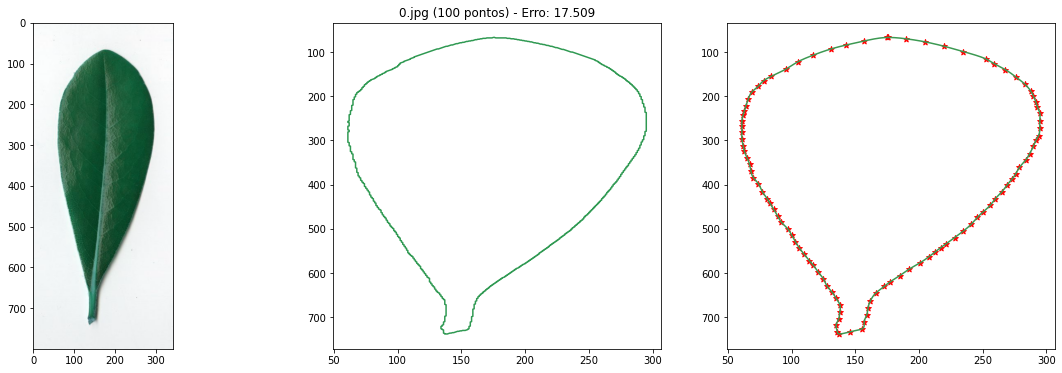
\includegraphics[width=0.9\textwidth]{img/res/0_100.png}
		\caption{Erro = 17.51.}
	\end{subfigure}
	\\
	\begin{subfigure}[b]{\textwidth}
		\centering
		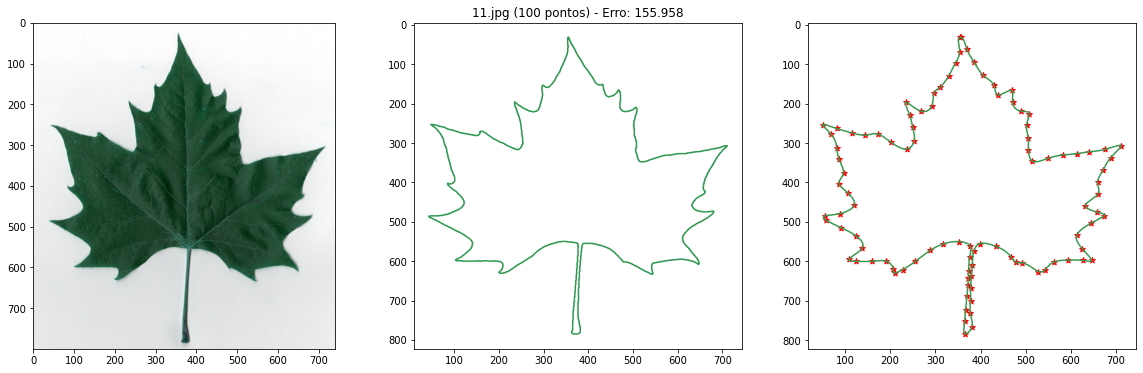
\includegraphics[width=0.9\textwidth]{img/res/1_100.png}
		\caption{Erro = 155.96.}
	\end{subfigure}
	\\
	\begin{subfigure}[b]{\textwidth}
		\centering
		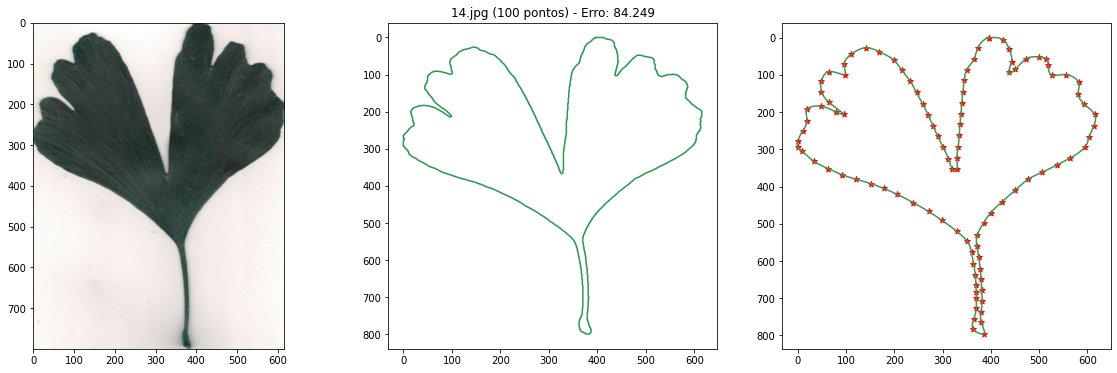
\includegraphics[width=0.9\textwidth]{img/res/2_100.png}
		\caption{Erro = 84.25.}
	\end{subfigure}
	\\
	\begin{subfigure}[b]{\textwidth}
		\centering
		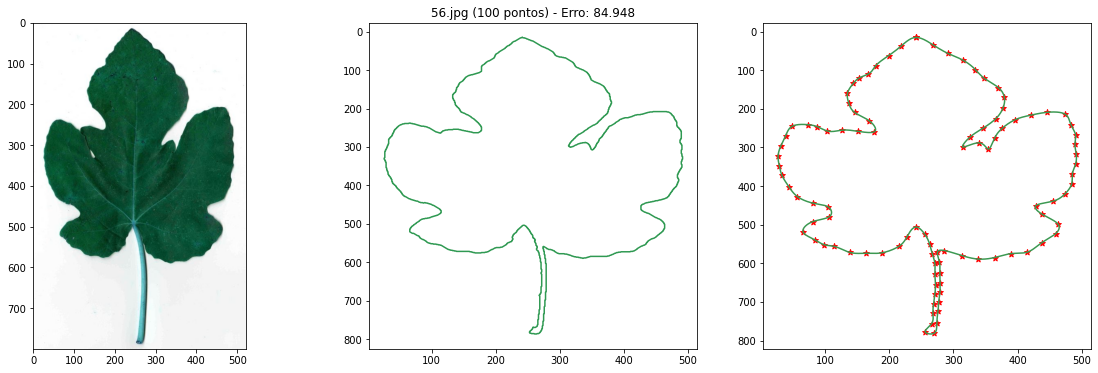
\includegraphics[width=0.9\textwidth]{img/res/3_100.png}
		\caption{Erro = 84.95.}
	\end{subfigure}
	\caption{Representação de folhas utilizando apenas 100 pontos como âncora.}
	\label{fig:folha3rep}
\end{figure}

As figuras \ref{fig:folha1rep}, \ref{fig:folha2rep} e \ref{fig:folha3rep} apresentam os resultados para quatro folhas distintas. Em cada uma delas, há 3 colunas: a primeira mostra a figura original, a segunda o contorno extraído e a terceira mostra a curva reconstruída, com os pontos âncora destacados com estrelas.

\subsection{Curvas abertas e em $\mathbb{R}^3$}

Outros testes foram realizados sobre curvas (discretizadas) abertas e fechadas, em domínios $\mathbb{R}^2$ e $\mathbb{R}^3$. De acordo com \citeonline{Sorkine2006}, o método de reconstrução funciona para quaisquer malhas que sejam aproximações lineares por partes de uma superfície suave.

A figura \ref{fig:c2d1} ilustra um exemplo de reconstrução de uma função paramétrica em $\mathbb{R}^2$ e fechada. A figura \ref{fig:c2d2} mostra um exemplo de função paramétrica em $\mathbb{R}^2$ e aberta. Em ambas, a figura à esquerda mostra a curva original, a do meio os pontos âncora escolhidos e a curva reconstruída a figura à direita.

\begin{figure}[H]
	\centering
	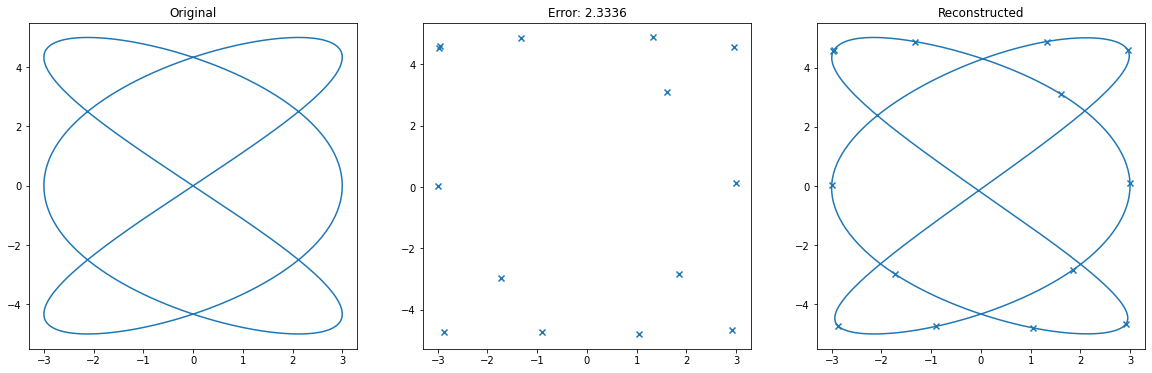
\includegraphics[width=1\textwidth]{img/res/closed2d.png}
	\caption{Representação da função paramétrica $(x(t), y(t)) = (3 cos(3t), 5sen(2t))$, com $t \in [0, 2\pi]$, utilizando 13 pontos como amostra.}
	\label{fig:c2d1}
\end{figure}

\begin{figure}[H]
	\centering
	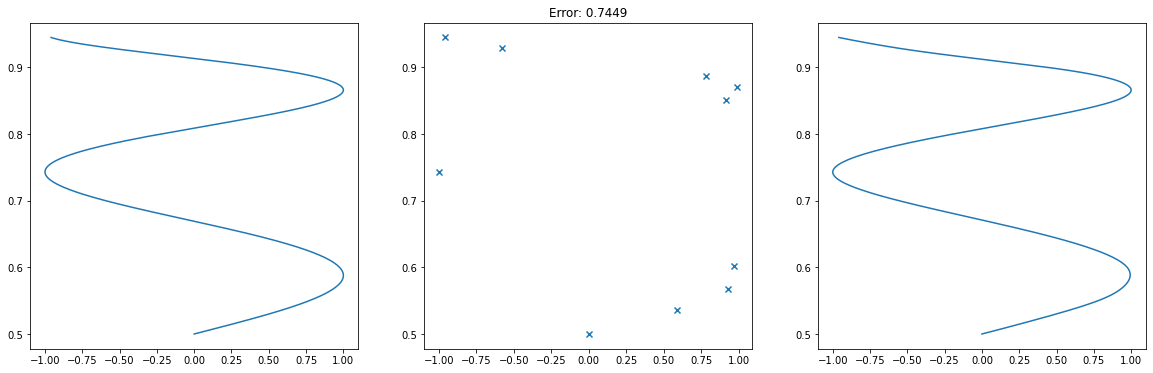
\includegraphics[width=1\textwidth]{img/res/open2d.png}
	\caption{Representação da função paramétrica $(x(t), y(t)) = (sin(5t), cos(t/3))$, com $t \in [1, \pi]$, utilizando 10 pontos como amostra.}
	\label{fig:c2d2}
\end{figure}

A figura \ref{fig:c3d1} mostra um exemplo de representação de uma curva paramétrica aberta em $\mathbb{R}^3$. A imagem à esquerda representa a curva original e a imagem à direita apresenta a curva reconstruída com os pontos âncora destacados. Neste caso, foram escolhidos pontos âncora linearmente espaçados.

\begin{figure}[H]
	\centering
	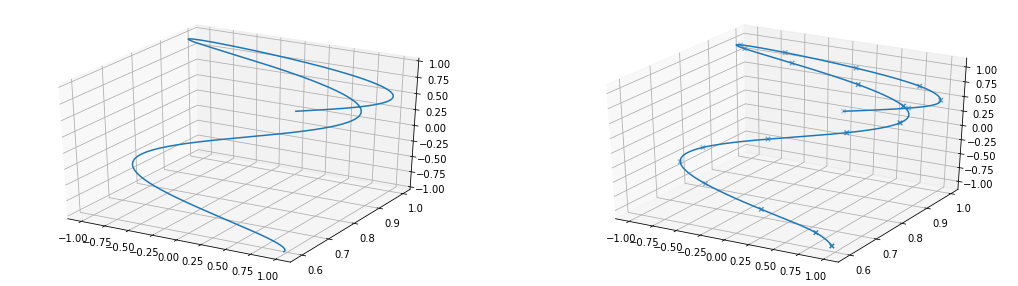
\includegraphics[width=1\textwidth]{img/res/open3d.png}
	\caption{Representação da função paramétrica $(x(t), y(t), z(t)) = (sin(3t), cos(t/5), sin(t))$, com $t \in [0, 1.5\pi]$, utilizando 20 pontos como amostra. Erro = 0.67.}
	\label{fig:c3d1}
\end{figure}

\subsection{Malhas poligonais}

Também foram realizados testes em malhas poligonais tridimensionais. Nestes exemplos, os pontos âncora foram escolhidos a partir de índices linearmente espaçados entre si. Por isso, pode-se destacar visualmente que alguns detalhes foram perdidos.

A figura \ref{fig:ex4rep} mostra exemplo de reconstrução na malha de um coelho utilizando-se apenas uma amostra dos pontos. A quantidade de pontos utilizadas em cada exemplo encontra-se na legenda de cada figura.

\begin{figure}[H]
	\centering
	\begin{subfigure}[b]{0.47\textwidth}
		\centering
		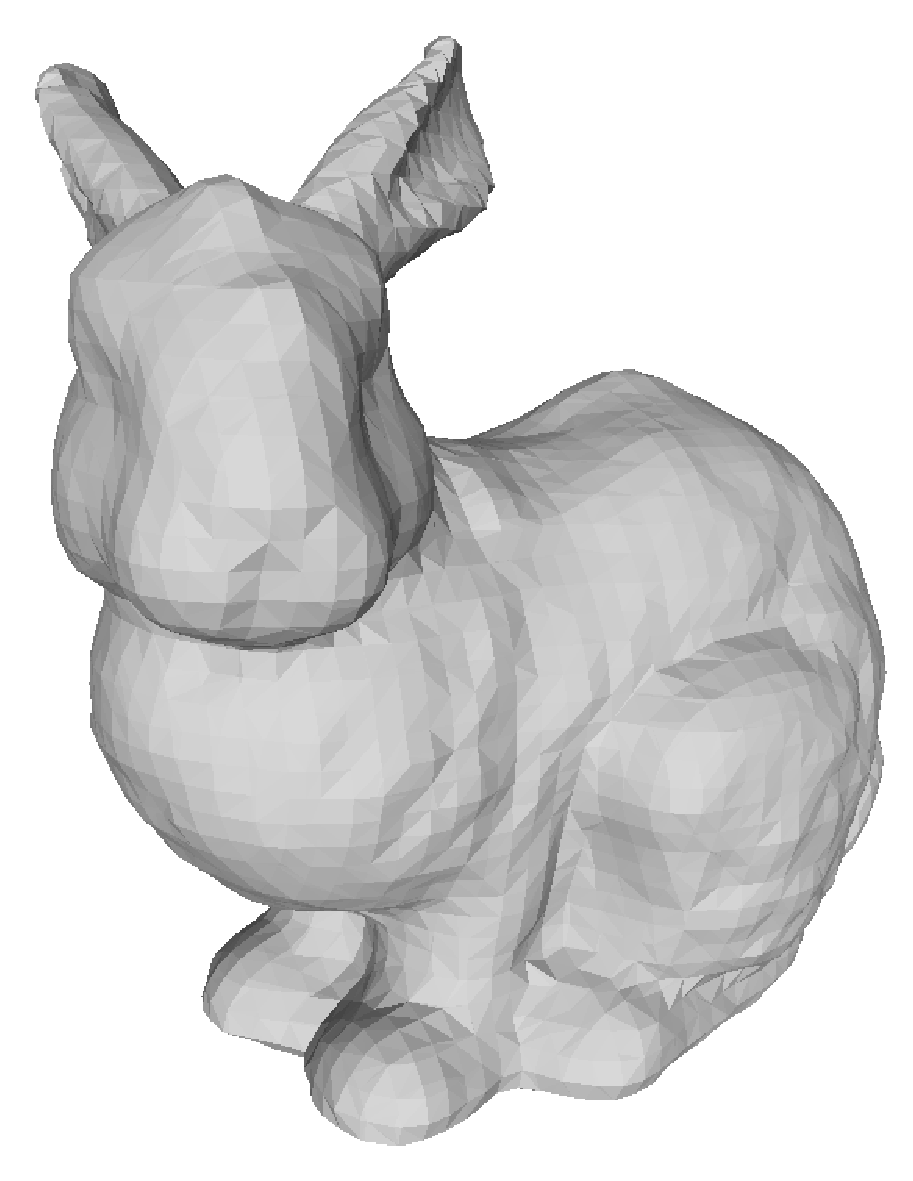
\includegraphics[width=0.43\textwidth]{img/res/bunny_all.eps}
		\caption{Malha original}
		\label{fig:ex41}
	\end{subfigure}
	\hfill
	\begin{subfigure}[b]{0.47\textwidth}
		\centering
		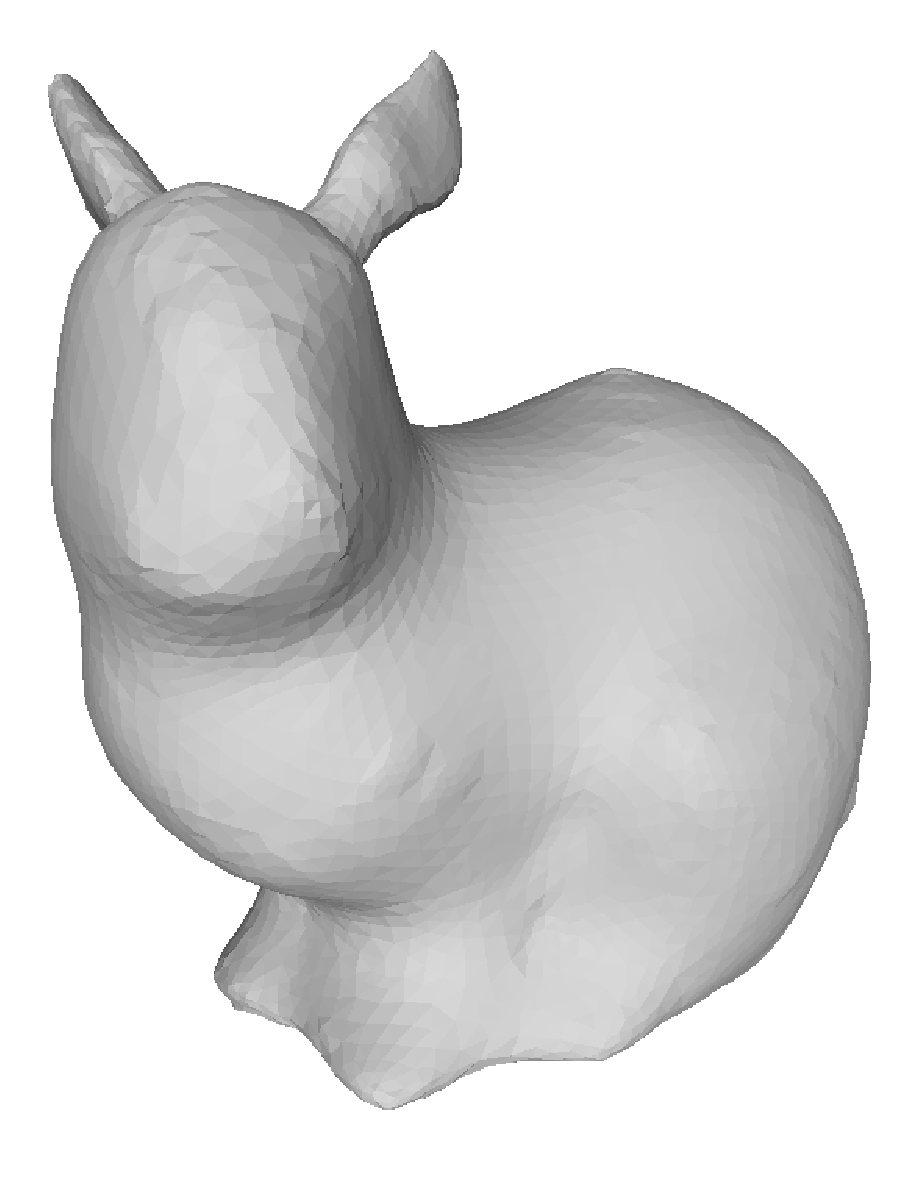
\includegraphics[width=0.43\textwidth]{img/res/bunny_10.eps}
		\caption{10\% dos pontos. Erro = 1037.08.}
		\label{fig:ex42}
	\end{subfigure}
	\\
	\begin{subfigure}[b]{0.47\textwidth}
		\centering
		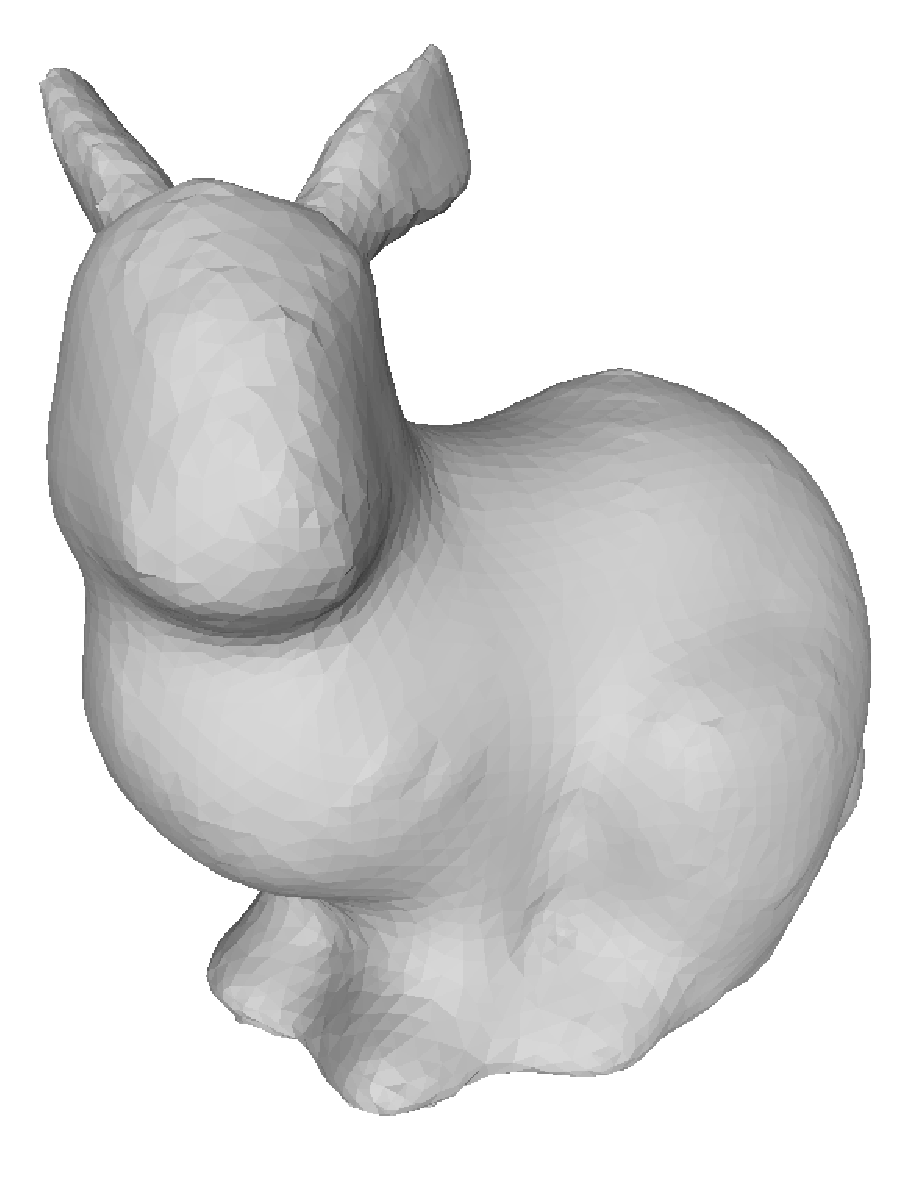
\includegraphics[width=0.43\textwidth]{img/res/bunny_30.eps}
		\caption{30\% dos pontos. Erro = 742.05.}
		\label{fig:ex43}
	\end{subfigure}
	\hfill
	\begin{subfigure}[b]{0.47\textwidth}
		\centering
		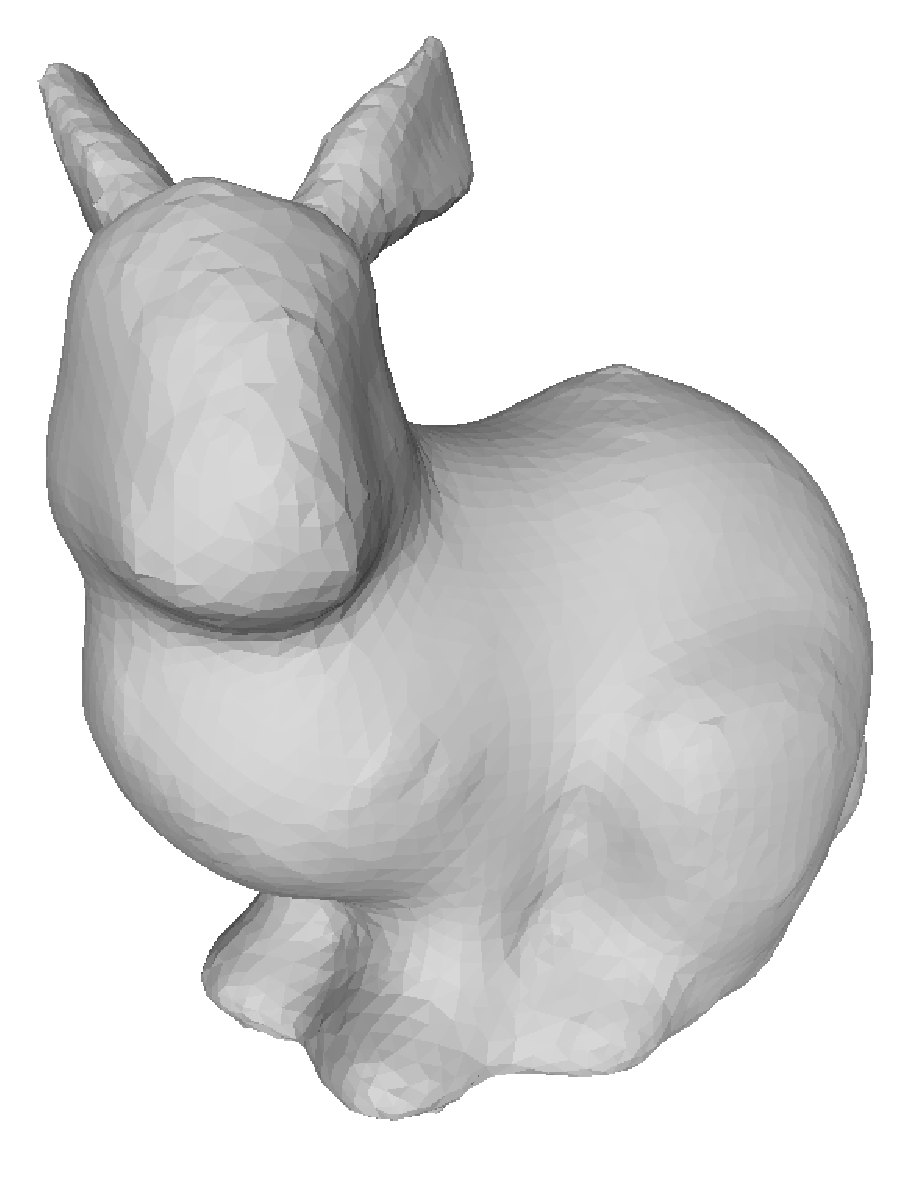
\includegraphics[width=0.43\textwidth]{img/res/bunny_50.eps}
		\caption{50\% dos pontos. Erro = 590.66.}
		\label{fig:ex44}
	\end{subfigure}
	\caption{Representação da malha de um coelho, utilizando apenas uma amostra dos pontos originais como âncoras.}
	\label{fig:ex4rep}
\end{figure}